\documentclass[1p]{elsarticle_modified}
%\bibliographystyle{elsarticle-num}

%\usepackage[colorlinks]{hyperref}
%\usepackage{abbrmath_seonhwa} %\Abb, \Ascr, \Acal ,\Abf, \Afrak
\usepackage{amsfonts}
\usepackage{amssymb}
\usepackage{amsmath}
\usepackage{amsthm}
\usepackage{scalefnt}
\usepackage{amsbsy}
\usepackage{kotex}
\usepackage{caption}
\usepackage{subfig}
\usepackage{color}
\usepackage{graphicx}
\usepackage{xcolor} %% white, black, red, green, blue, cyan, magenta, yellow
\usepackage{float}
\usepackage{setspace}
\usepackage{hyperref}

\usepackage{tikz}
\usetikzlibrary{arrows}

\usepackage{multirow}
\usepackage{array} % fixed length table
\usepackage{hhline}

%%%%%%%%%%%%%%%%%%%%%
\makeatletter
\renewcommand*\env@matrix[1][\arraystretch]{%
	\edef\arraystretch{#1}%
	\hskip -\arraycolsep
	\let\@ifnextchar\new@ifnextchar
	\array{*\c@MaxMatrixCols c}}
\makeatother %https://tex.stackexchange.com/questions/14071/how-can-i-increase-the-line-spacing-in-a-matrix
%%%%%%%%%%%%%%%

\usepackage[normalem]{ulem}

\newcommand{\msout}[1]{\ifmmode\text{\sout{\ensuremath{#1}}}\else\sout{#1}\fi}
%SOURCE: \msout is \stkout macro in https://tex.stackexchange.com/questions/20609/strikeout-in-math-mode

\newcommand{\cancel}[1]{
	\ifmmode
	{\color{red}\msout{#1}}
	\else
	{\color{red}\sout{#1}}
	\fi
}

\newcommand{\add}[1]{
	{\color{blue}\uwave{#1}}
}

\newcommand{\replace}[2]{
	\ifmmode
	{\color{red}\msout{#1}}{\color{blue}\uwave{#2}}
	\else
	{\color{red}\sout{#1}}{\color{blue}\uwave{#2}}
	\fi
}

\newcommand{\Sol}{\mathcal{S}} %segment
\newcommand{\D}{D} %diagram
\newcommand{\A}{\mathcal{A}} %arc


%%%%%%%%%%%%%%%%%%%%%%%%%%%%%5 test

\def\sl{\operatorname{\textup{SL}}(2,\Cbb)}
\def\psl{\operatorname{\textup{PSL}}(2,\Cbb)}
\def\quan{\mkern 1mu \triangleright \mkern 1mu}

\theoremstyle{definition}
\newtheorem{thm}{Theorem}[section]
\newtheorem{prop}[thm]{Proposition}
\newtheorem{lem}[thm]{Lemma}
\newtheorem{ques}[thm]{Question}
\newtheorem{cor}[thm]{Corollary}
\newtheorem{defn}[thm]{Definition}
\newtheorem{exam}[thm]{Example}
\newtheorem{rmk}[thm]{Remark}
\newtheorem{alg}[thm]{Algorithm}

\newcommand{\I}{\sqrt{-1}}
\begin{document}

%\begin{frontmatter}
%
%\title{Boundary parabolic representations of knots up to 8 crossings}
%
%%% Group authors per affiliation:
%\author{Yunhi Cho} 
%\address{Department of Mathematics, University of Seoul, Seoul, Korea}
%\ead{yhcho@uos.ac.kr}
%
%
%\author{Seonhwa Kim} %\fnref{s_kim}}
%\address{Center for Geometry and Physics, Institute for Basic Science, Pohang, 37673, Korea}
%\ead{ryeona17@ibs.re.kr}
%
%\author{Hyuk Kim}
%\address{Department of Mathematical Sciences, Seoul National University, Seoul 08826, Korea}
%\ead{hyukkim@snu.ac.kr}
%
%\author{Seokbeom Yoon}
%\address{Department of Mathematical Sciences, Seoul National University, Seoul, 08826,  Korea}
%\ead{sbyoon15@snu.ac.kr}
%
%\begin{abstract}
%We find all boundary parabolic representation of knots up to 8 crossings.
%
%\end{abstract}
%\begin{keyword}
%    \MSC[2010] 57M25 
%\end{keyword}
%
%\end{frontmatter}

%\linenumbers
%\tableofcontents
%
\newcommand\colored[1]{\textcolor{white}{\rule[-0.35ex]{0.8em}{1.4ex}}\kern-0.8em\color{red} #1}%
%\newcommand\colored[1]{\textcolor{white}{ #1}\kern-2.17ex	\textcolor{white}{ #1}\kern-1.81ex	\textcolor{white}{ #1}\kern-2.15ex\color{red}#1	}

{\Large $\underline{12n_{0038}~(K12n_{0038})}$}

\setlength{\tabcolsep}{10pt}
\renewcommand{\arraystretch}{1.6}
\vspace{1cm}\begin{tabular}{m{100pt}>{\centering\arraybackslash}m{274pt}}
\multirow{5}{120pt}{
	\centering
	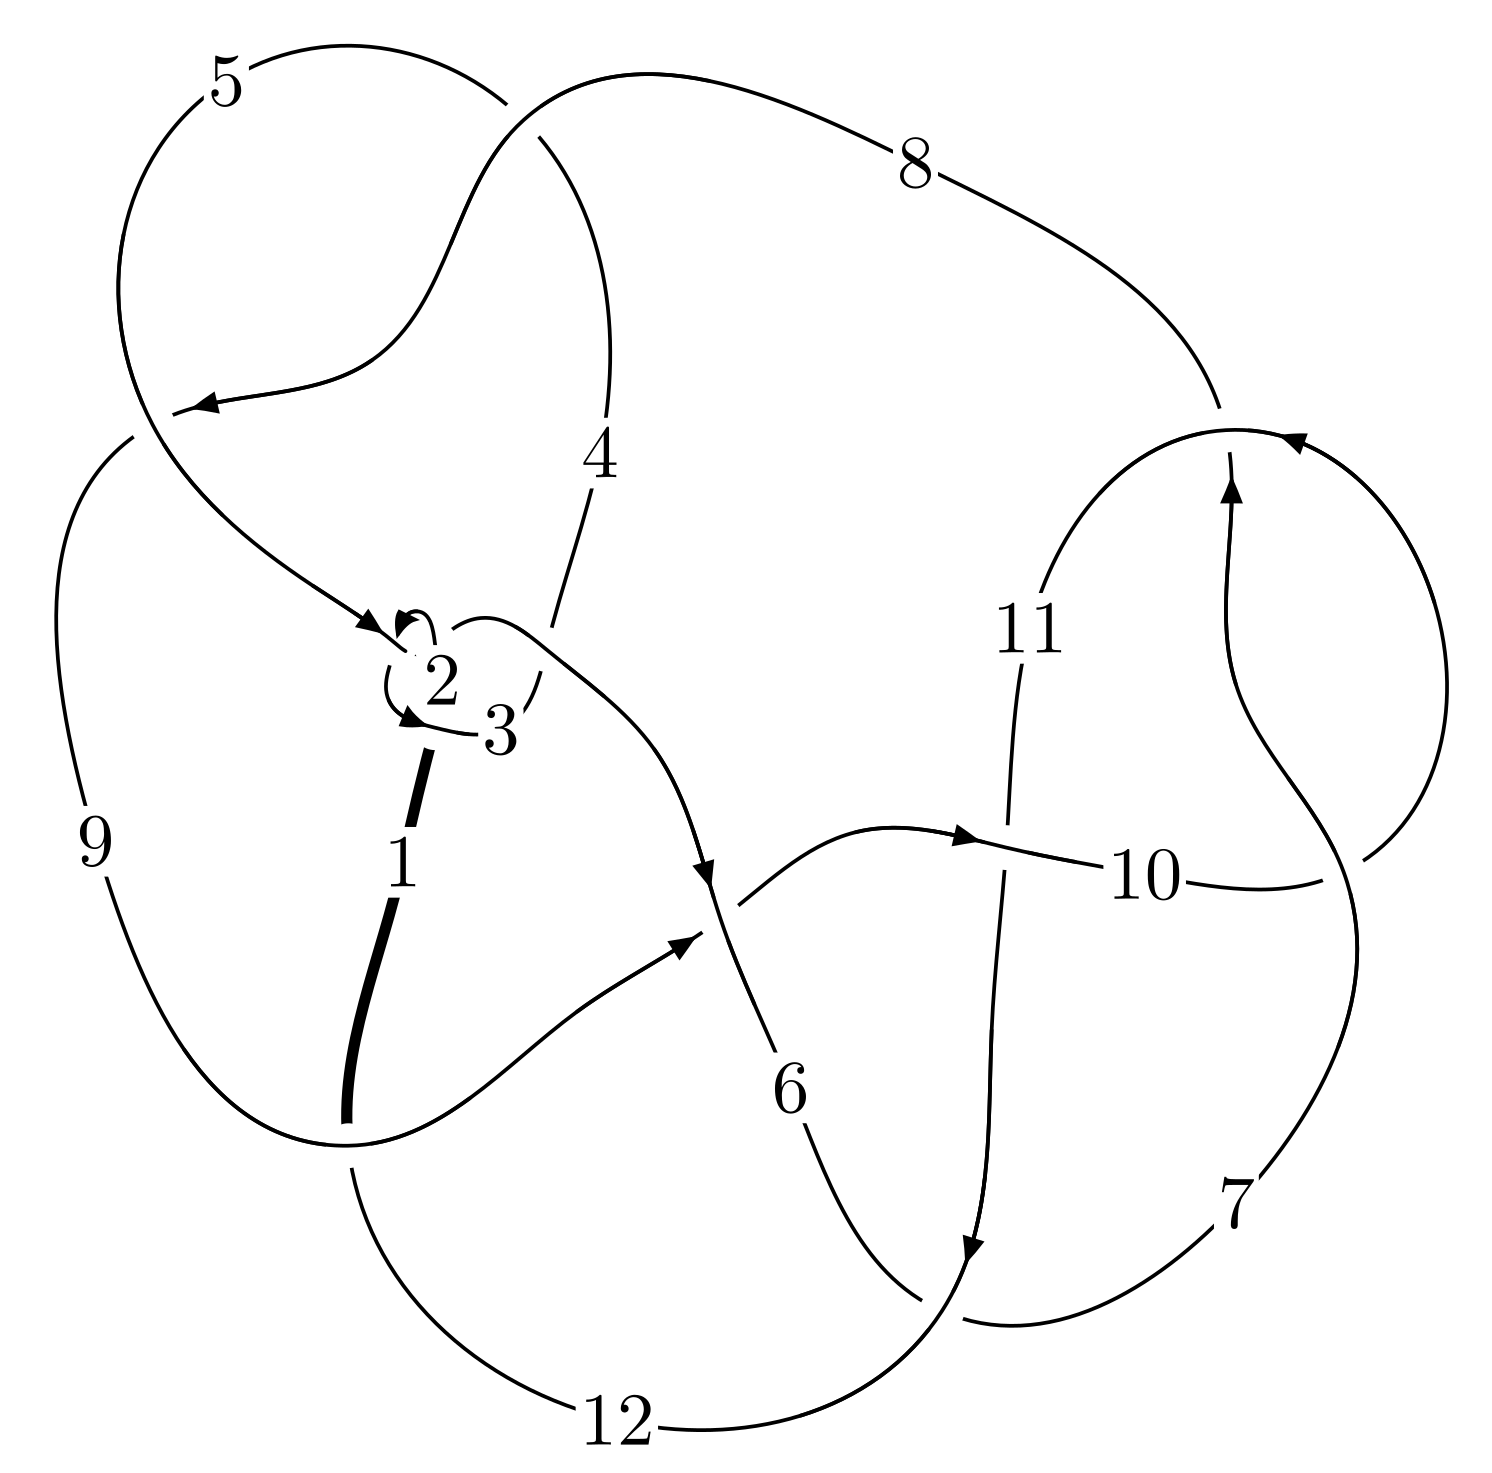
\includegraphics[width=112pt]{../../../GIT/diagram.site/Diagrams/png/2127_12n_0038.png}\\
\ \ \ A knot diagram\footnotemark}&
\allowdisplaybreaks
\textbf{Linearized knot diagam} \\
\cline{2-2}
 &
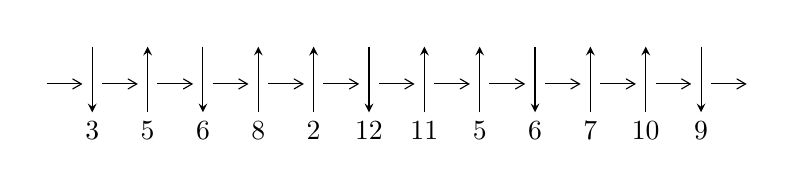
\begin{tikzpicture}[x=20pt, y=17pt]
	% nodes
	\node (C0) at (0, 0) {};
	\node (C1) at (1, 0) {};
	\node (C1U) at (1, +1) {};
	\node (C1D) at (1, -1) {3};

	\node (C2) at (2, 0) {};
	\node (C2U) at (2, +1) {};
	\node (C2D) at (2, -1) {5};

	\node (C3) at (3, 0) {};
	\node (C3U) at (3, +1) {};
	\node (C3D) at (3, -1) {6};

	\node (C4) at (4, 0) {};
	\node (C4U) at (4, +1) {};
	\node (C4D) at (4, -1) {8};

	\node (C5) at (5, 0) {};
	\node (C5U) at (5, +1) {};
	\node (C5D) at (5, -1) {2};

	\node (C6) at (6, 0) {};
	\node (C6U) at (6, +1) {};
	\node (C6D) at (6, -1) {12};

	\node (C7) at (7, 0) {};
	\node (C7U) at (7, +1) {};
	\node (C7D) at (7, -1) {11};

	\node (C8) at (8, 0) {};
	\node (C8U) at (8, +1) {};
	\node (C8D) at (8, -1) {5};

	\node (C9) at (9, 0) {};
	\node (C9U) at (9, +1) {};
	\node (C9D) at (9, -1) {6};

	\node (C10) at (10, 0) {};
	\node (C10U) at (10, +1) {};
	\node (C10D) at (10, -1) {7};

	\node (C11) at (11, 0) {};
	\node (C11U) at (11, +1) {};
	\node (C11D) at (11, -1) {10};

	\node (C12) at (12, 0) {};
	\node (C12U) at (12, +1) {};
	\node (C12D) at (12, -1) {9};
	\node (C13) at (13, 0) {};

	% arrows
	\draw[->,>={angle 60}]
	(C0) edge (C1) (C1) edge (C2) (C2) edge (C3) (C3) edge (C4) (C4) edge (C5) (C5) edge (C6) (C6) edge (C7) (C7) edge (C8) (C8) edge (C9) (C9) edge (C10) (C10) edge (C11) (C11) edge (C12) (C12) edge (C13) ;	\draw[->,>=stealth]
	(C1U) edge (C1D) (C2D) edge (C2U) (C3U) edge (C3D) (C4D) edge (C4U) (C5D) edge (C5U) (C6U) edge (C6D) (C7D) edge (C7U) (C8D) edge (C8U) (C9U) edge (C9D) (C10D) edge (C10U) (C11D) edge (C11U) (C12U) edge (C12D) ;
	\end{tikzpicture} \\
\hhline{~~} \\& 
\textbf{Solving Sequence} \\ \cline{2-2} 
 &
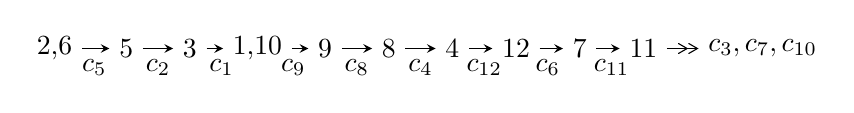
\begin{tikzpicture}[x=23pt, y=7pt]
	% node
	\node (A0) at (-1/8, 0) {2,6};
	\node (A1) at (1, 0) {5};
	\node (A2) at (2, 0) {3};
	\node (A3) at (49/16, 0) {1,10};
	\node (A4) at (33/8, 0) {9};
	\node (A5) at (41/8, 0) {8};
	\node (A6) at (49/8, 0) {4};
	\node (A7) at (57/8, 0) {12};
	\node (A8) at (65/8, 0) {7};
	\node (A9) at (73/8, 0) {11};
	\node (C1) at (1/2, -1) {$c_{5}$};
	\node (C2) at (3/2, -1) {$c_{2}$};
	\node (C3) at (5/2, -1) {$c_{1}$};
	\node (C4) at (29/8, -1) {$c_{9}$};
	\node (C5) at (37/8, -1) {$c_{8}$};
	\node (C6) at (45/8, -1) {$c_{4}$};
	\node (C7) at (53/8, -1) {$c_{12}$};
	\node (C8) at (61/8, -1) {$c_{6}$};
	\node (C9) at (69/8, -1) {$c_{11}$};
	\node (A10) at (11, 0) {$c_{3},c_{7},c_{10}$};

	% edge
	\draw[->,>=stealth]	
	(A0) edge (A1) (A1) edge (A2) (A2) edge (A3) (A3) edge (A4) (A4) edge (A5) (A5) edge (A6) (A6) edge (A7) (A7) edge (A8) (A8) edge (A9) ;
	\draw[->>,>={angle 60}]	
	(A9) edge (A10);
\end{tikzpicture} \\ 

\end{tabular} \\

\footnotetext{
The image of knot diagram is generated by the software ``\textbf{Draw programme}" developed by Andrew Bartholomew(\url{http://www.layer8.co.uk/maths/draw/index.htm\#Running-draw}), where we modified some parts for our purpose(\url{https://github.com/CATsTAILs/LinksPainter}).
}\phantom \\ \newline 
\centering \textbf{Ideals for irreducible components\footnotemark of $X_{\text{par}}$} 
 
\begin{align*}
I^u_{1}&=\langle 
132 u^{44}+811 u^{43}+\cdots+32 b+15,\;-275 u^{44}-1867 u^{43}+\cdots+32 a+615,\;u^{45}+7 u^{44}+\cdots-5 u-1\rangle \\
I^u_{2}&=\langle 
- a u+3 b+2 a,\;a^6- a^5 u- a^5-3 a^4 u+12 a^3 u-6 a^3-9 a u+18 a-27,\;u^2- u+1\rangle \\
\\
\end{align*}
\raggedright * 2 irreducible components of $\dim_{\mathbb{C}}=0$, with total 57 representations.\\
\footnotetext{All coefficients of polynomials are rational numbers. But the coefficients are sometimes approximated in decimal forms when there is not enough margin.}
\newpage
\renewcommand{\arraystretch}{1}
\centering \section*{I. $I^u_{1}= \langle 132 u^{44}+811 u^{43}+\cdots+32 b+15,\;-275 u^{44}-1867 u^{43}+\cdots+32 a+615,\;u^{45}+7 u^{44}+\cdots-5 u-1 \rangle$}
\flushleft \textbf{(i) Arc colorings}\\
\begin{tabular}{m{7pt} m{180pt} m{7pt} m{180pt} }
\flushright $a_{2}=$&$\begin{pmatrix}0\\u\end{pmatrix}$ \\
\flushright $a_{6}=$&$\begin{pmatrix}1\\0\end{pmatrix}$ \\
\flushright $a_{5}=$&$\begin{pmatrix}1\\u^2\end{pmatrix}$ \\
\flushright $a_{3}=$&$\begin{pmatrix}u\\u^3+u\end{pmatrix}$ \\
\flushright $a_{1}=$&$\begin{pmatrix}u^3\\u^5+u^3+u\end{pmatrix}$ \\
\flushright $a_{10}=$&$\begin{pmatrix}8.59375 u^{44}+58.3438 u^{43}+\cdots-80.9688 u-19.2188\\-4.12500 u^{44}-25.3438 u^{43}+\cdots+14.5625 u-0.468750\end{pmatrix}$ \\
\flushright $a_{9}=$&$\begin{pmatrix}4.46875 u^{44}+33 u^{43}+\cdots-66.4063 u-19.6875\\-4.12500 u^{44}-25.3438 u^{43}+\cdots+14.5625 u-0.468750\end{pmatrix}$ \\
\flushright $a_{8}=$&$\begin{pmatrix}5.59375 u^{44}+40.8125 u^{43}+\cdots-67.9063 u-17.5000\\-5.06250 u^{44}-32.0313 u^{43}+\cdots+15.3750 u-0.531250\end{pmatrix}$ \\
\flushright $a_{4}=$&$\begin{pmatrix}- u^3\\u^3+u\end{pmatrix}$ \\
\flushright $a_{12}=$&$\begin{pmatrix}\frac{1}{32} u^{43}+\frac{3}{16} u^{42}+\cdots-\frac{17}{8} u+\frac{31}{32}\\-0.0312500 u^{44}-0.218750 u^{43}+\cdots+0.156250 u+0.0312500\end{pmatrix}$ \\
\flushright $a_{7}=$&$\begin{pmatrix}-0.468750 u^{44}-3.31250 u^{43}+\cdots+2.71875 u+1.56250\\0.468750 u^{44}+2.84375 u^{43}+\cdots-0.656250 u-0.0312500\end{pmatrix}$ \\
\flushright $a_{11}=$&$\begin{pmatrix}0.812500 u^{44}+5.40625 u^{43}+\cdots-4.25000 u-0.593750\\-0.468750 u^{44}-2.90625 u^{43}+\cdots+1.90625 u+0.0937500\end{pmatrix}$\\&\end{tabular}
\flushleft \textbf{(ii) Obstruction class $= -1$}\\~\\
\flushleft \textbf{(iii) Cusp Shapes $= -\frac{177}{16} u^{44}-\frac{1121}{16} u^{43}+\cdots+\frac{1137}{16} u+\frac{95}{8}$}\\~\\
\newpage\renewcommand{\arraystretch}{1}
\flushleft \textbf{(iv) u-Polynomials at the component}\newline \\
\begin{tabular}{m{50pt}|m{274pt}}
Crossings & \hspace{64pt}u-Polynomials at each crossing \\
\hline $$\begin{aligned}c_{1}\end{aligned}$$&$\begin{aligned}
&u^{45}+9 u^{44}+\cdots-9 u-1
\end{aligned}$\\
\hline $$\begin{aligned}c_{2},c_{5}\end{aligned}$$&$\begin{aligned}
&u^{45}+7 u^{44}+\cdots-5 u-1
\end{aligned}$\\
\hline $$\begin{aligned}c_{3}\end{aligned}$$&$\begin{aligned}
&u^{45}-7 u^{44}+\cdots-877615 u-93361
\end{aligned}$\\
\hline $$\begin{aligned}c_{4},c_{8}\end{aligned}$$&$\begin{aligned}
&u^{45}- u^{44}+\cdots+8192 u-4096
\end{aligned}$\\
\hline $$\begin{aligned}c_{6}\end{aligned}$$&$\begin{aligned}
&u^{45}-9 u^{44}+\cdots+203 u-37
\end{aligned}$\\
\hline $$\begin{aligned}c_{7},c_{10}\end{aligned}$$&$\begin{aligned}
&u^{45}-3 u^{44}+\cdots+3 u-1
\end{aligned}$\\
\hline $$\begin{aligned}c_{9}\end{aligned}$$&$\begin{aligned}
&u^{45}+3 u^{44}+\cdots+2181 u-1201
\end{aligned}$\\
\hline $$\begin{aligned}c_{11}\end{aligned}$$&$\begin{aligned}
&u^{45}-23 u^{44}+\cdots+3 u-1
\end{aligned}$\\
\hline $$\begin{aligned}c_{12}\end{aligned}$$&$\begin{aligned}
&u^{45}- u^{44}+\cdots+3 u-1
\end{aligned}$\\
\hline
\end{tabular}\\~\\
\newpage\renewcommand{\arraystretch}{1}
\flushleft \textbf{(v) Riley Polynomials at the component}\newline \\
\begin{tabular}{m{50pt}|m{274pt}}
Crossings & \hspace{64pt}Riley Polynomials at each crossing \\
\hline $$\begin{aligned}c_{1}\end{aligned}$$&$\begin{aligned}
&y^{45}+61 y^{44}+\cdots-29 y-1
\end{aligned}$\\
\hline $$\begin{aligned}c_{2},c_{5}\end{aligned}$$&$\begin{aligned}
&y^{45}+9 y^{44}+\cdots-9 y-1
\end{aligned}$\\
\hline $$\begin{aligned}c_{3}\end{aligned}$$&$\begin{aligned}
&y^{45}+113 y^{44}+\cdots-304227830897 y-8716276321
\end{aligned}$\\
\hline $$\begin{aligned}c_{4},c_{8}\end{aligned}$$&$\begin{aligned}
&y^{45}-65 y^{44}+\cdots+33554432 y-16777216
\end{aligned}$\\
\hline $$\begin{aligned}c_{6}\end{aligned}$$&$\begin{aligned}
&y^{45}+21 y^{44}+\cdots+14347 y-1369
\end{aligned}$\\
\hline $$\begin{aligned}c_{7},c_{10}\end{aligned}$$&$\begin{aligned}
&y^{45}-23 y^{44}+\cdots+3 y-1
\end{aligned}$\\
\hline $$\begin{aligned}c_{9}\end{aligned}$$&$\begin{aligned}
&y^{45}+17 y^{44}+\cdots+9246099 y-1442401
\end{aligned}$\\
\hline $$\begin{aligned}c_{11}\end{aligned}$$&$\begin{aligned}
&y^{45}+y^{44}+\cdots+11 y-1
\end{aligned}$\\
\hline $$\begin{aligned}c_{12}\end{aligned}$$&$\begin{aligned}
&y^{45}+77 y^{44}+\cdots+3 y-1
\end{aligned}$\\
\hline
\end{tabular}\\~\\
\newpage\flushleft \textbf{(vi) Complex Volumes and Cusp Shapes}
$$\begin{array}{c|c|c}  
\text{Solutions to }I^u_{1}& \I (\text{vol} + \sqrt{-1}CS) & \text{Cusp shape}\\
 \hline 
\begin{aligned}
u &= \phantom{-}0.865449 + 0.454219 I \\
a &= \phantom{-}0.319220 + 0.531227 I \\
b &= -0.36863 - 1.46260 I\end{aligned}
 & \phantom{-}4.73623 - 2.35998 I & \phantom{-}8.35847 + 1.71921 I \\ \hline\begin{aligned}
u &= \phantom{-}0.865449 - 0.454219 I \\
a &= \phantom{-}0.319220 - 0.531227 I \\
b &= -0.36863 + 1.46260 I\end{aligned}
 & \phantom{-}4.73623 + 2.35998 I & \phantom{-}8.35847 - 1.71921 I \\ \hline\begin{aligned}
u &= \phantom{-}0.330564 + 0.971277 I \\
a &= -1.35737 - 1.01368 I \\
b &= \phantom{-}0.526140 + 0.066430 I\end{aligned}
 & -1.15352 + 2.68830 I & -0.34175 - 6.47696 I \\ \hline\begin{aligned}
u &= \phantom{-}0.330564 - 0.971277 I \\
a &= -1.35737 + 1.01368 I \\
b &= \phantom{-}0.526140 - 0.066430 I\end{aligned}
 & -1.15352 - 2.68830 I & -0.34175 + 6.47696 I \\ \hline\begin{aligned}
u &= \phantom{-}0.622281 + 0.846945 I \\
a &= -0.079868 + 0.698124 I \\
b &= -0.493189 - 0.089540 I\end{aligned}
 & \phantom{-}0.80407 + 2.44032 I & \phantom{-}0.39786 - 3.53339 I \\ \hline\begin{aligned}
u &= \phantom{-}0.622281 - 0.846945 I \\
a &= -0.079868 - 0.698124 I \\
b &= -0.493189 + 0.089540 I\end{aligned}
 & \phantom{-}0.80407 - 2.44032 I & \phantom{-}0.39786 + 3.53339 I \\ \hline\begin{aligned}
u &= \phantom{-}0.755037 + 0.558570 I \\
a &= -0.0783721 - 0.0338596 I \\
b &= -0.107622 + 0.976039 I\end{aligned}
 & \phantom{-}1.57242 + 1.53241 I & \phantom{-}4.30562 - 2.68000 I \\ \hline\begin{aligned}
u &= \phantom{-}0.755037 - 0.558570 I \\
a &= -0.0783721 + 0.0338596 I \\
b &= -0.107622 - 0.976039 I\end{aligned}
 & \phantom{-}1.57242 - 1.53241 I & \phantom{-}4.30562 + 2.68000 I \\ \hline\begin{aligned}
u &= \phantom{-}0.867507 + 0.624607 I \\
a &= -0.382914 + 0.278991 I \\
b &= \phantom{-}0.56116 - 1.43284 I\end{aligned}
 & \phantom{-}4.57167 + 5.62351 I & \phantom{-}7.47380 - 5.91915 I \\ \hline\begin{aligned}
u &= \phantom{-}0.867507 - 0.624607 I \\
a &= -0.382914 - 0.278991 I \\
b &= \phantom{-}0.56116 + 1.43284 I\end{aligned}
 & \phantom{-}4.57167 - 5.62351 I & \phantom{-}7.47380 + 5.91915 I\\
 \hline 
 \end{array}$$\newpage$$\begin{array}{c|c|c}  
\text{Solutions to }I^u_{1}& \I (\text{vol} + \sqrt{-1}CS) & \text{Cusp shape}\\
 \hline 
\begin{aligned}
u &= \phantom{-}0.180988 + 0.903067 I \\
a &= \phantom{-}0.74445 + 1.99166 I \\
b &= -0.201660 - 0.527398 I\end{aligned}
 & \phantom{-}0.112526 - 1.116170 I & \phantom{-}0.739301 + 0.318022 I \\ \hline\begin{aligned}
u &= \phantom{-}0.180988 - 0.903067 I \\
a &= \phantom{-}0.74445 - 1.99166 I \\
b &= -0.201660 + 0.527398 I\end{aligned}
 & \phantom{-}0.112526 + 1.116170 I & \phantom{-}0.739301 - 0.318022 I \\ \hline\begin{aligned}
u &= \phantom{-}0.482106 + 1.053890 I \\
a &= -1.78297 + 0.42437 I \\
b &= \phantom{-}0.516649 - 0.731743 I\end{aligned}
 & -0.20453 + 3.20330 I & \phantom{-0.000000 } 0. - 3.29559 I \\ \hline\begin{aligned}
u &= \phantom{-}0.482106 - 1.053890 I \\
a &= -1.78297 - 0.42437 I \\
b &= \phantom{-}0.516649 + 0.731743 I\end{aligned}
 & -0.20453 - 3.20330 I & \phantom{-0.000000 -}0. + 3.29559 I \\ \hline\begin{aligned}
u &= \phantom{-}0.601778 + 1.060200 I \\
a &= \phantom{-}1.28241 - 1.47156 I \\
b &= \phantom{-}0.110511 + 1.232230 I\end{aligned}
 & \phantom{-}3.02293 - 0.08785 I & \phantom{-0.000000 } 0 \\ \hline\begin{aligned}
u &= \phantom{-}0.601778 - 1.060200 I \\
a &= \phantom{-}1.28241 + 1.47156 I \\
b &= \phantom{-}0.110511 - 1.232230 I\end{aligned}
 & \phantom{-}3.02293 + 0.08785 I & \phantom{-0.000000 } 0 \\ \hline\begin{aligned}
u &= \phantom{-}0.503909 + 1.128940 I \\
a &= \phantom{-}2.43305 - 0.92945 I \\
b &= -0.80290 + 1.19457 I\end{aligned}
 & \phantom{-}2.36444 + 7.52477 I & \phantom{-0.000000 } 0 \\ \hline\begin{aligned}
u &= \phantom{-}0.503909 - 1.128940 I \\
a &= \phantom{-}2.43305 + 0.92945 I \\
b &= -0.80290 - 1.19457 I\end{aligned}
 & \phantom{-}2.36444 - 7.52477 I & \phantom{-0.000000 } 0 \\ \hline\begin{aligned}
u &= -0.084493 + 0.713012 I \\
a &= -1.01316 + 2.46838 I \\
b &= \phantom{-}0.821961 - 0.446891 I\end{aligned}
 & -0.81007 + 4.73637 I & -1.24888 - 6.79408 I \\ \hline\begin{aligned}
u &= -0.084493 - 0.713012 I \\
a &= -1.01316 - 2.46838 I \\
b &= \phantom{-}0.821961 + 0.446891 I\end{aligned}
 & -0.81007 - 4.73637 I & -1.24888 + 6.79408 I\\
 \hline 
 \end{array}$$\newpage$$\begin{array}{c|c|c}  
\text{Solutions to }I^u_{1}& \I (\text{vol} + \sqrt{-1}CS) & \text{Cusp shape}\\
 \hline 
\begin{aligned}
u &= -0.921571 + 0.928254 I \\
a &= \phantom{-}0.300181 - 0.167382 I \\
b &= \phantom{-}0.141408 - 0.815178 I\end{aligned}
 & \phantom{-}7.46078 - 0.75691 I & \phantom{-0.000000 } 0 \\ \hline\begin{aligned}
u &= -0.921571 - 0.928254 I \\
a &= \phantom{-}0.300181 + 0.167382 I \\
b &= \phantom{-}0.141408 + 0.815178 I\end{aligned}
 & \phantom{-}7.46078 + 0.75691 I & \phantom{-0.000000 } 0 \\ \hline\begin{aligned}
u &= -0.904820 + 0.965905 I \\
a &= -0.790239 + 0.408383 I \\
b &= \phantom{-}0.376118 + 0.820565 I\end{aligned}
 & \phantom{-}7.34035 - 5.98505 I & \phantom{-0.000000 } 0 \\ \hline\begin{aligned}
u &= -0.904820 - 0.965905 I \\
a &= -0.790239 - 0.408383 I \\
b &= \phantom{-}0.376118 - 0.820565 I\end{aligned}
 & \phantom{-}7.34035 + 5.98505 I & \phantom{-0.000000 } 0 \\ \hline\begin{aligned}
u &= -1.009740 + 0.883218 I \\
a &= -0.377537 + 0.824899 I \\
b &= \phantom{-}1.22594 - 1.41286 I\end{aligned}
 & \phantom{-}10.71020 + 1.37563 I & \phantom{-0.000000 } 0 \\ \hline\begin{aligned}
u &= -1.009740 - 0.883218 I \\
a &= -0.377537 - 0.824899 I \\
b &= \phantom{-}1.22594 + 1.41286 I\end{aligned}
 & \phantom{-}10.71020 - 1.37563 I & \phantom{-0.000000 } 0 \\ \hline\begin{aligned}
u &= -1.034420 + 0.865842 I \\
a &= \phantom{-}0.664407 - 1.034480 I \\
b &= -1.61121 + 1.49060 I\end{aligned}
 & \phantom{-}13.5421 + 6.5266 I & \phantom{-0.000000 } 0 \\ \hline\begin{aligned}
u &= -1.034420 - 0.865842 I \\
a &= \phantom{-}0.664407 + 1.034480 I \\
b &= -1.61121 - 1.49060 I\end{aligned}
 & \phantom{-}13.5421 - 6.5266 I & \phantom{-0.000000 } 0 \\ \hline\begin{aligned}
u &= -0.387424 + 0.500589 I \\
a &= -1.93597 + 1.18940 I \\
b &= \phantom{-}1.225780 + 0.662919 I\end{aligned}
 & \phantom{-}0.14562 - 6.62336 I & \phantom{-}2.53824 + 3.24872 I \\ \hline\begin{aligned}
u &= -0.387424 - 0.500589 I \\
a &= -1.93597 - 1.18940 I \\
b &= \phantom{-}1.225780 - 0.662919 I\end{aligned}
 & \phantom{-}0.14562 + 6.62336 I & \phantom{-}2.53824 - 3.24872 I\\
 \hline 
 \end{array}$$\newpage$$\begin{array}{c|c|c}  
\text{Solutions to }I^u_{1}& \I (\text{vol} + \sqrt{-1}CS) & \text{Cusp shape}\\
 \hline 
\begin{aligned}
u &= -1.024940 + 0.925322 I \\
a &= -0.086100 - 1.156550 I \\
b &= -0.91727 + 1.93981 I\end{aligned}
 & \phantom{-}15.3464 - 2.2779 I & \phantom{-0.000000 } 0 \\ \hline\begin{aligned}
u &= -1.024940 - 0.925322 I \\
a &= -0.086100 + 1.156550 I \\
b &= -0.91727 - 1.93981 I\end{aligned}
 & \phantom{-}15.3464 + 2.2779 I & \phantom{-0.000000 } 0 \\ \hline\begin{aligned}
u &= -0.128241 + 0.602764 I \\
a &= \phantom{-}1.33735 - 2.06079 I \\
b &= -0.899761 + 0.098160 I\end{aligned}
 & -2.43287 + 0.11880 I & -4.07087 - 1.28262 I \\ \hline\begin{aligned}
u &= -0.128241 - 0.602764 I \\
a &= \phantom{-}1.33735 + 2.06079 I \\
b &= -0.899761 - 0.098160 I\end{aligned}
 & -2.43287 - 0.11880 I & -4.07087 + 1.28262 I \\ \hline\begin{aligned}
u &= -0.911280 + 1.044170 I \\
a &= -1.97485 + 0.39149 I \\
b &= \phantom{-}1.36520 + 1.26824 I\end{aligned}
 & \phantom{-}10.17040 - 8.40766 I & \phantom{-0.000000 } 0 \\ \hline\begin{aligned}
u &= -0.911280 - 1.044170 I \\
a &= -1.97485 - 0.39149 I \\
b &= \phantom{-}1.36520 - 1.26824 I\end{aligned}
 & \phantom{-}10.17040 + 8.40766 I & \phantom{-0.000000 } 0 \\ \hline\begin{aligned}
u &= -0.907943 + 1.066410 I \\
a &= \phantom{-}2.33785 - 0.47875 I \\
b &= -1.69979 - 1.31179 I\end{aligned}
 & \phantom{-}12.8666 - 13.6205 I & \phantom{-0.000000 } 0 \\ \hline\begin{aligned}
u &= -0.907943 - 1.066410 I \\
a &= \phantom{-}2.33785 + 0.47875 I \\
b &= -1.69979 + 1.31179 I\end{aligned}
 & \phantom{-}12.8666 + 13.6205 I & \phantom{-0.000000 } 0 \\ \hline\begin{aligned}
u &= -0.948740 + 1.039640 I \\
a &= \phantom{-}1.92604 + 0.22525 I \\
b &= -1.11708 - 1.78219 I\end{aligned}
 & \phantom{-}14.9563 - 4.9353 I & \phantom{-0.000000 } 0 \\ \hline\begin{aligned}
u &= -0.948740 - 1.039640 I \\
a &= \phantom{-}1.92604 - 0.22525 I \\
b &= -1.11708 + 1.78219 I\end{aligned}
 & \phantom{-}14.9563 + 4.9353 I & \phantom{-0.000000 } 0\\
 \hline 
 \end{array}$$\newpage$$\begin{array}{c|c|c}  
\text{Solutions to }I^u_{1}& \I (\text{vol} + \sqrt{-1}CS) & \text{Cusp shape}\\
 \hline 
\begin{aligned}
u &= -0.306772 + 0.492284 I \\
a &= \phantom{-}1.74185 - 1.46922 I \\
b &= -1.089070 - 0.461342 I\end{aligned}
 & -1.91688 - 1.75082 I & -1.56719 - 0.68553 I \\ \hline\begin{aligned}
u &= -0.306772 - 0.492284 I \\
a &= \phantom{-}1.74185 + 1.46922 I \\
b &= -1.089070 + 0.461342 I\end{aligned}
 & -1.91688 + 1.75082 I & -1.56719 + 0.68553 I \\ \hline\begin{aligned}
u &= \phantom{-}0.455358\phantom{ +0.000000I} \\
a &= -1.30613\phantom{ +0.000000I} \\
b &= \phantom{-}0.610269\phantom{ +0.000000I}\end{aligned}
 & \phantom{-}1.30638\phantom{ +0.000000I} & \phantom{-}7.75970\phantom{ +0.000000I} \\ \hline\begin{aligned}
u &= -0.366917 + 0.266389 I \\
a &= -1.07439 + 1.09771 I \\
b &= \phantom{-}0.632186 + 0.840901 I\end{aligned}
 & \phantom{-}2.23991 + 0.49049 I & \phantom{-}6.10667 - 1.43657 I \\ \hline\begin{aligned}
u &= -0.366917 - 0.266389 I \\
a &= -1.07439 - 1.09771 I \\
b &= \phantom{-}0.632186 - 0.840901 I\end{aligned}
 & \phantom{-}2.23991 - 0.49049 I & \phantom{-}6.10667 + 1.43657 I\\
 \hline 
 \end{array}$$\newpage\newpage\renewcommand{\arraystretch}{1}
\centering \section*{II. $I^u_{2}= \langle - a u+3 b+2 a,\;- a^5 u-3 a^4 u+\cdots+18 a-27,\;u^2- u+1 \rangle$}
\flushleft \textbf{(i) Arc colorings}\\
\begin{tabular}{m{7pt} m{180pt} m{7pt} m{180pt} }
\flushright $a_{2}=$&$\begin{pmatrix}0\\u\end{pmatrix}$ \\
\flushright $a_{6}=$&$\begin{pmatrix}1\\0\end{pmatrix}$ \\
\flushright $a_{5}=$&$\begin{pmatrix}1\\u-1\end{pmatrix}$ \\
\flushright $a_{3}=$&$\begin{pmatrix}u\\u-1\end{pmatrix}$ \\
\flushright $a_{1}=$&$\begin{pmatrix}-1\\0\end{pmatrix}$ \\
\flushright $a_{10}=$&$\begin{pmatrix}a\\\frac{1}{3} a u-\frac{2}{3} a\end{pmatrix}$ \\
\flushright $a_{9}=$&$\begin{pmatrix}\frac{1}{3} a u+\frac{1}{3} a\\\frac{1}{3} a u-\frac{2}{3} a\end{pmatrix}$ \\
\flushright $a_{8}=$&$\begin{pmatrix}\frac{1}{3} a u+\frac{1}{3} a\\\frac{1}{3} a u-\frac{2}{3} a\end{pmatrix}$ \\
\flushright $a_{4}=$&$\begin{pmatrix}1\\u-1\end{pmatrix}$ \\
\flushright $a_{12}=$&$\begin{pmatrix}-\frac{1}{3} a^2-1\\-\frac{1}{3} a^2 u+\frac{1}{3} a^2\end{pmatrix}$ \\
\flushright $a_{7}=$&$\begin{pmatrix}\frac{1}{9} a^4 u+\frac{1}{3} a^2 u+\cdots-\frac{1}{3} a^2+1\\-\frac{1}{9} a^4 u\end{pmatrix}$ \\
\flushright $a_{11}=$&$\begin{pmatrix}\frac{2}{9} a^4 u-\frac{1}{3} a^2 u+\cdots+\frac{1}{3} a^2-1\\-\frac{1}{9} a^4 u\end{pmatrix}$\\&\end{tabular}
\flushleft \textbf{(ii) Obstruction class $= 1$}\\~\\
\flushleft \textbf{(iii) Cusp Shapes $= \frac{2}{27} a^5 u-\frac{1}{27} a^5-\frac{4}{9} a^4 u-\frac{2}{9} a^3 u+\frac{4}{9} a^3+a^2 u-\frac{5}{3} a^2-2 a u+2 a-3 u+6$}\\~\\
\newpage\renewcommand{\arraystretch}{1}
\flushleft \textbf{(iv) u-Polynomials at the component}\newline \\
\begin{tabular}{m{50pt}|m{274pt}}
Crossings & \hspace{64pt}u-Polynomials at each crossing \\
\hline $$\begin{aligned}c_{1},c_{3},c_{5}\end{aligned}$$&$\begin{aligned}
&(u^2- u+1)^6
\end{aligned}$\\
\hline $$\begin{aligned}c_{2}\end{aligned}$$&$\begin{aligned}
&(u^2+u+1)^6
\end{aligned}$\\
\hline $$\begin{aligned}c_{4},c_{8}\end{aligned}$$&$\begin{aligned}
&u^{12}
\end{aligned}$\\
\hline $$\begin{aligned}c_{6},c_{11}\end{aligned}$$&$\begin{aligned}
&(u^6-3 u^5+5 u^4-4 u^3+2 u^2- u+1)^2
\end{aligned}$\\
\hline $$\begin{aligned}c_{7},c_{9},c_{12}\end{aligned}$$&$\begin{aligned}
&(u^6- u^5- u^4+2 u^3- u+1)^2
\end{aligned}$\\
\hline $$\begin{aligned}c_{10}\end{aligned}$$&$\begin{aligned}
&(u^6+u^5- u^4-2 u^3+u+1)^2
\end{aligned}$\\
\hline
\end{tabular}\\~\\
\newpage\renewcommand{\arraystretch}{1}
\flushleft \textbf{(v) Riley Polynomials at the component}\newline \\
\begin{tabular}{m{50pt}|m{274pt}}
Crossings & \hspace{64pt}Riley Polynomials at each crossing \\
\hline $$\begin{aligned}c_{1},c_{2},c_{3}\\c_{5}\end{aligned}$$&$\begin{aligned}
&(y^2+y+1)^6
\end{aligned}$\\
\hline $$\begin{aligned}c_{4},c_{8}\end{aligned}$$&$\begin{aligned}
&y^{12}
\end{aligned}$\\
\hline $$\begin{aligned}c_{6},c_{11}\end{aligned}$$&$\begin{aligned}
&(y^6+y^5+5 y^4+6 y^2+3 y+1)^2
\end{aligned}$\\
\hline $$\begin{aligned}c_{7},c_{9},c_{10}\\c_{12}\end{aligned}$$&$\begin{aligned}
&(y^6-3 y^5+5 y^4-4 y^3+2 y^2- y+1)^2
\end{aligned}$\\
\hline
\end{tabular}\\~\\
\newpage\flushleft \textbf{(vi) Complex Volumes and Cusp Shapes}
$$\begin{array}{c|c|c}  
\text{Solutions to }I^u_{2}& \I (\text{vol} + \sqrt{-1}CS) & \text{Cusp shape}\\
 \hline 
\begin{aligned}
u &= \phantom{-}0.500000 + 0.866025 I \\
a &= \phantom{-}0.066864 + 1.367670 I \\
b &= -0.428243 - 0.664531 I\end{aligned}
 & \phantom{-}1.89061 + 1.10558 I & \phantom{-}3.50232 - 2.57477 I \\ \hline\begin{aligned}
u &= \phantom{-}0.500000 + 0.866025 I \\
a &= \phantom{-}1.217870 - 0.625927 I \\
b &= -0.428243 + 0.664531 I\end{aligned}
 & \phantom{-}1.89061 + 2.95419 I & \phantom{-}7.01188 - 5.05114 I \\ \hline\begin{aligned}
u &= \phantom{-}0.500000 + 0.866025 I \\
a &= -1.24734 - 1.31124 I \\
b &= \phantom{-}1.002190 + 0.295542 I\end{aligned}
 & -1.89061 + 1.10558 I & \phantom{-}0.06995 - 2.75005 I \\ \hline\begin{aligned}
u &= \phantom{-}0.500000 + 0.866025 I \\
a &= -1.75924 - 0.42461 I \\
b &= \phantom{-}1.002190 - 0.295542 I\end{aligned}
 & -1.89061 + 2.95419 I & -1.81693 - 4.43387 I \\ \hline\begin{aligned}
u &= \phantom{-}0.500000 + 0.866025 I \\
a &= \phantom{-}2.09482 + 0.09194 I \\
b &= -1.073950 + 0.558752 I\end{aligned}
 & \phantom{-0.000000 } -3.66314 I & \phantom{-}4.13964 + 1.97785 I \\ \hline\begin{aligned}
u &= \phantom{-}0.500000 + 0.866025 I \\
a &= \phantom{-}1.12703 + 1.76820 I \\
b &= -1.073950 - 0.558752 I\end{aligned}
 & \phantom{-0.000000 -}7.72290 I & \phantom{-}1.09315 - 9.68468 I \\ \hline\begin{aligned}
u &= \phantom{-}0.500000 - 0.866025 I \\
a &= \phantom{-}0.066864 - 1.367670 I \\
b &= -0.428243 + 0.664531 I\end{aligned}
 & \phantom{-}1.89061 - 1.10558 I & \phantom{-}3.50232 + 2.57477 I \\ \hline\begin{aligned}
u &= \phantom{-}0.500000 - 0.866025 I \\
a &= \phantom{-}1.217870 + 0.625927 I \\
b &= -0.428243 - 0.664531 I\end{aligned}
 & \phantom{-}1.89061 - 2.95419 I & \phantom{-}7.01188 + 5.05114 I \\ \hline\begin{aligned}
u &= \phantom{-}0.500000 - 0.866025 I \\
a &= -1.24734 + 1.31124 I \\
b &= \phantom{-}1.002190 - 0.295542 I\end{aligned}
 & -1.89061 - 1.10558 I & \phantom{-}0.06995 + 2.75005 I \\ \hline\begin{aligned}
u &= \phantom{-}0.500000 - 0.866025 I \\
a &= -1.75924 + 0.42461 I \\
b &= \phantom{-}1.002190 + 0.295542 I\end{aligned}
 & -1.89061 - 2.95419 I & -1.81693 + 4.43387 I\\
 \hline 
 \end{array}$$\newpage$$\begin{array}{c|c|c}  
\text{Solutions to }I^u_{2}& \I (\text{vol} + \sqrt{-1}CS) & \text{Cusp shape}\\
 \hline 
\begin{aligned}
u &= \phantom{-}0.500000 - 0.866025 I \\
a &= \phantom{-}2.09482 - 0.09194 I \\
b &= -1.073950 - 0.558752 I\end{aligned}
 & \phantom{-0.000000 -}3.66314 I & \phantom{-}4.13964 - 1.97785 I \\ \hline\begin{aligned}
u &= \phantom{-}0.500000 - 0.866025 I \\
a &= \phantom{-}1.12703 - 1.76820 I \\
b &= -1.073950 + 0.558752 I\end{aligned}
 & \phantom{-0.000000 } -7.72290 I & \phantom{-}1.09315 + 9.68468 I\\
 \hline 
 \end{array}$$\newpage
\newpage\renewcommand{\arraystretch}{1}
\centering \section*{ III. u-Polynomials}
\begin{tabular}{m{50pt}|m{274pt}}
Crossings & \hspace{64pt}u-Polynomials at each crossing \\
\hline $$\begin{aligned}c_{1}\end{aligned}$$&$\begin{aligned}
&((u^2- u+1)^6)(u^{45}+9 u^{44}+\cdots-9 u-1)
\end{aligned}$\\
\hline $$\begin{aligned}c_{2}\end{aligned}$$&$\begin{aligned}
&((u^2+u+1)^6)(u^{45}+7 u^{44}+\cdots-5 u-1)
\end{aligned}$\\
\hline $$\begin{aligned}c_{3}\end{aligned}$$&$\begin{aligned}
&((u^2- u+1)^6)(u^{45}-7 u^{44}+\cdots-877615 u-93361)
\end{aligned}$\\
\hline $$\begin{aligned}c_{4},c_{8}\end{aligned}$$&$\begin{aligned}
&u^{12}(u^{45}- u^{44}+\cdots+8192 u-4096)
\end{aligned}$\\
\hline $$\begin{aligned}c_{5}\end{aligned}$$&$\begin{aligned}
&((u^2- u+1)^6)(u^{45}+7 u^{44}+\cdots-5 u-1)
\end{aligned}$\\
\hline $$\begin{aligned}c_{6}\end{aligned}$$&$\begin{aligned}
&((u^6-3 u^5+5 u^4-4 u^3+2 u^2- u+1)^{2})(u^{45}-9 u^{44}+\cdots+203 u-37)
\end{aligned}$\\
\hline $$\begin{aligned}c_{7}\end{aligned}$$&$\begin{aligned}
&((u^6- u^5- u^4+2 u^3- u+1)^2)(u^{45}-3 u^{44}+\cdots+3 u-1)
\end{aligned}$\\
\hline $$\begin{aligned}c_{9}\end{aligned}$$&$\begin{aligned}
&((u^6- u^5- u^4+2 u^3- u+1)^2)(u^{45}+3 u^{44}+\cdots+2181 u-1201)
\end{aligned}$\\
\hline $$\begin{aligned}c_{10}\end{aligned}$$&$\begin{aligned}
&((u^6+u^5- u^4-2 u^3+u+1)^2)(u^{45}-3 u^{44}+\cdots+3 u-1)
\end{aligned}$\\
\hline $$\begin{aligned}c_{11}\end{aligned}$$&$\begin{aligned}
&((u^6-3 u^5+5 u^4-4 u^3+2 u^2- u+1)^{2})(u^{45}-23 u^{44}+\cdots+3 u-1)
\end{aligned}$\\
\hline $$\begin{aligned}c_{12}\end{aligned}$$&$\begin{aligned}
&((u^6- u^5- u^4+2 u^3- u+1)^2)(u^{45}- u^{44}+\cdots+3 u-1)
\end{aligned}$\\
\hline
\end{tabular}\newpage\renewcommand{\arraystretch}{1}
\centering \section*{ IV. Riley Polynomials}
\begin{tabular}{m{50pt}|m{274pt}}
Crossings & \hspace{64pt}Riley Polynomials at each crossing \\
\hline $$\begin{aligned}c_{1}\end{aligned}$$&$\begin{aligned}
&((y^2+y+1)^6)(y^{45}+61 y^{44}+\cdots-29 y-1)
\end{aligned}$\\
\hline $$\begin{aligned}c_{2},c_{5}\end{aligned}$$&$\begin{aligned}
&((y^2+y+1)^6)(y^{45}+9 y^{44}+\cdots-9 y-1)
\end{aligned}$\\
\hline $$\begin{aligned}c_{3}\end{aligned}$$&$\begin{aligned}
&((y^2+y+1)^6)(y^{45}+113 y^{44}+\cdots-3.04228\times10^{11} y-8.71628\times10^{9})
\end{aligned}$\\
\hline $$\begin{aligned}c_{4},c_{8}\end{aligned}$$&$\begin{aligned}
&y^{12}(y^{45}-65 y^{44}+\cdots+3.35544\times10^{7} y-1.67772\times10^{7})
\end{aligned}$\\
\hline $$\begin{aligned}c_{6}\end{aligned}$$&$\begin{aligned}
&((y^6+y^5+5 y^4+6 y^2+3 y+1)^2)(y^{45}+21 y^{44}+\cdots+14347 y-1369)
\end{aligned}$\\
\hline $$\begin{aligned}c_{7},c_{10}\end{aligned}$$&$\begin{aligned}
&((y^6-3 y^5+5 y^4-4 y^3+2 y^2- y+1)^{2})(y^{45}-23 y^{44}+\cdots+3 y-1)
\end{aligned}$\\
\hline $$\begin{aligned}c_{9}\end{aligned}$$&$\begin{aligned}
&(y^6-3 y^5+5 y^4-4 y^3+2 y^2- y+1)^2\\
&\cdot(y^{45}+17 y^{44}+\cdots+9246099 y-1442401)
\end{aligned}$\\
\hline $$\begin{aligned}c_{11}\end{aligned}$$&$\begin{aligned}
&((y^6+y^5+5 y^4+6 y^2+3 y+1)^2)(y^{45}+y^{44}+\cdots+11 y-1)
\end{aligned}$\\
\hline $$\begin{aligned}c_{12}\end{aligned}$$&$\begin{aligned}
&((y^6-3 y^5+5 y^4-4 y^3+2 y^2- y+1)^{2})(y^{45}+77 y^{44}+\cdots+3 y-1)
\end{aligned}$\\
\hline
\end{tabular}
\vskip 2pc
\end{document}